\documentclass[pdftex]{article}
\usepackage[T1]{fontenc}
\usepackage[utf8]{inputenc}
\usepackage{graphicx}
\usepackage[font=scriptsize,labelfont=bf]{caption}
\usepackage{titling}

\setlength{\droptitle}{-15em}
\title{PHYS 721 Homework 7}
\author{Nick Tyler}
\date{}


\begin{document}
\captionsetup[figure]{aboveskip=-15pt}
\captionsetup[figure]{belowskip=15pt}
\maketitle
\begin{enumerate}
	\item  By fitting a function to the data there appears to be a few regions where the data
			is above the background function especially in the region around $126.5 \: GeV.$
			When investigrating this region further by fitting a Gausian function with a mean
			around $126.5 \: GeV$ a peak apears with a mass of $126.32 \pm 0.66 \: GeV$ and a
			width of $0.97 \pm 0.13 \: GeV$ with a $\chi^{2}$ value close to $1.$\

		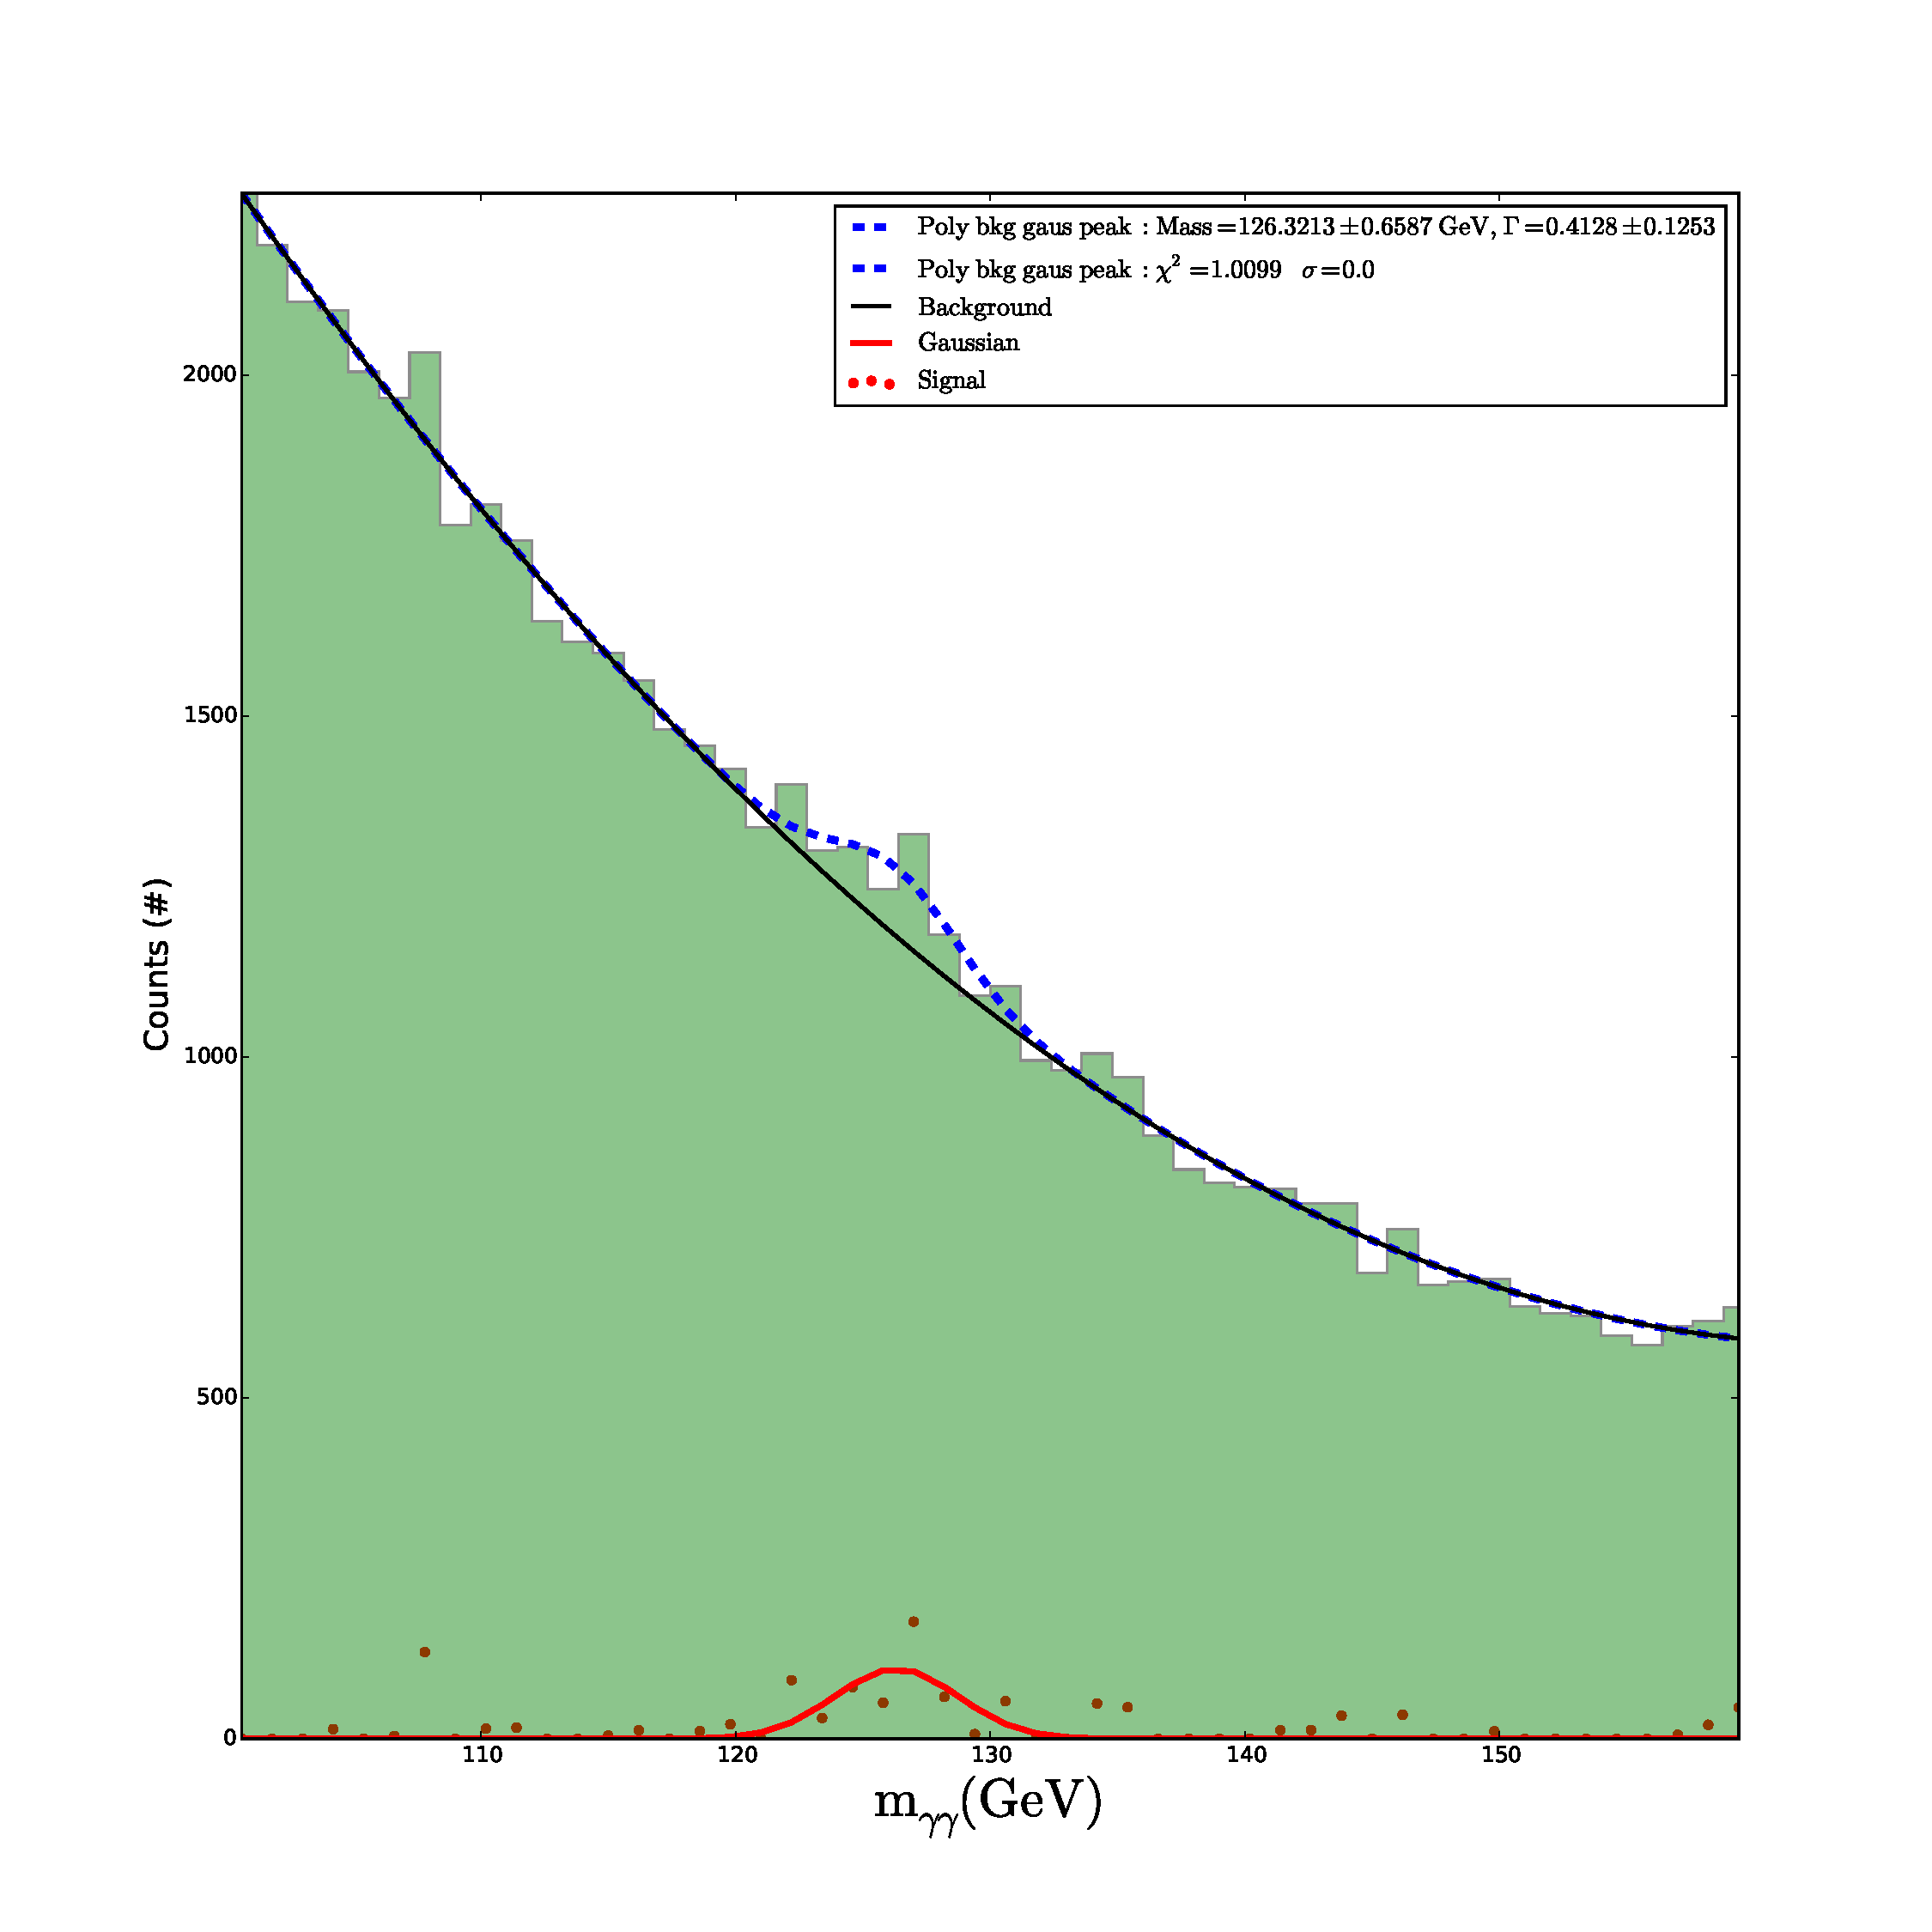
\includegraphics[scale=0.35]{Problem_1.pdf}\\
		\captionof{figure}{Shows the mass of $\gamma \gamma$ pairs with a background function fit
				as well as a gausian peak fit on the background. In red the subtracted signal as well 
				as subtracted Gausian function can also be seen.}

	\item Given that the width is $1.66 \: GeV$ without any knowledge of the mass gives
			a signifigance of 


\end{enumerate}

\end{document}
